\chapter{Usando estilos de página predefinidos}
A maneira mais fácil de criar cabeçalhos e rodapés personalizados com scrlayer-scrpage é usar um dos estilos de página predefinidos.

\begin{verbatim}
    \pagestyle{scrheadings}
    \pagestyle{plain.scrheadings} 
\end{verbatim}

O pacote scrlayer-scrpage fornece dois estilos de página que você pode reconfigurar conforme sua preferência.

O primeiro estilo de página é \textbf{scrheadings}, que é pretendido como um estilo de página com títulos correntes. Seus padrões são semelhantes aos títulos de estilo de página das classes \LaTeX\ ou \KOMAScript\ padrão. Você pode configurar exatamente o que aparece no cabeçalho ou rodapé com os comandos e opções descritos abaixo.

O segundo estilo de página é \textbf{plain.scrheadings}, que é pretendido como um estilo sem título corrente. Seus padrões se assemelham aos do estilo de página simples das classes padrão ou \KOMAScript. Você pode configurar exatamente o que aparece no cabeçalho ou rodapé com os comandos e opções descritos abaixo.

Você pode, é claro, configurar scrheadings para ser um estilo de página sem um título corrente e plain.scrheadings para ser um estilo de página com um título corrente. No entanto, é aconselhável aderir às convenções mencionadas acima. Os dois estilos de página influenciam mutuamente um ao outro. Depois de aplicar um desses estilos de página, scrheadings se tornará acessível como headings e o estilo de página plain.scrheadings se tornará acessível como plain. Assim, se você usar uma classe ou pacote que alterna automaticamente entre headings e plain, você só precisa selecionar scrheadings ou plain.scrheadings uma vez. Patches diretos para as classes ou pacotes correspondentes não são necessários. Este par de estilos de página pode, portanto, servir como um substituto imediato para headings e plain. Se você precisar de mais pares como este, consulte a seção 18.2 na parte II.
\begin{verbatim}
    \lehead[plain.scrheadings content ]{scrheadings content}
    \cehead[plain.scrheadings content ]{scrheadings content}
    \rehead[plain.scrheadings content ]{scrheadings content}
    \lohead[plain.scrheadings content ]{scrheadings content}
    \cohead[plain.scrheadings content ]{scrheadings content}
    \rohead[plain.scrheadings content ]{scrheadings content}
\end{verbatim}

Você pode definir o conteúdo do cabeçalho para os estilos de página plain.scrheadings e scrheadings com esses comandos. O argumento opcional define o conteúdo de um elemento do estilo de página plain.scrheadings, enquanto o argumento obrigatório define o conteúdo do elemento correspondente do estilo de página scrheadings.

O conteúdo de páginas pares — ou à esquerda — pode ser definido com \verb|\lehead|, \verb|\cehead| e \verb|\rehead|. O “e” que aparece como a segunda letra dos nomes dos comandos significa “par”.

O conteúdo de páginas ímpares — ou à direita — pode ser definido com \verb|\lohead|, \verb|\cohead| e \verb|\rohead|. O “o” que aparece como a segunda letra dos nomes dos comandos significa “ímpar”.

Observe que na impressão de um lado, existem apenas páginas à direita, e o \LaTeX\ as designa como páginas ímpares, independentemente do número da página.

Cada cabeçalho consiste em um elemento alinhado à esquerda que pode ser definido com \verb|\lehead| ou \verb|\lohead|.

O “l” que aparece como a primeira letra dos nomes dos comandos significa “alinhado à esquerda”.

Da mesma forma, cada cabeçalho tem um elemento centralizado que pode ser definido com \verb|\cehead| ou \verb|\cohead|. O “c” que aparece como a primeira letra dos nomes dos comandos significa “centralizado”.

E, também, cada cabeçalho tem um elemento alinhado à direita que pode ser definido com \verb|\rehead| ou \verb|\rohead|.

O “r” que aparece como a primeira letra dos nomes dos comandos significa “alinhado à direita”.

Esses elementos não têm atributos de fonte individuais que você pode alterar usando os comandos \cmd{set\-ko\-ma\-font} e \cmd{add\-to\-ko\-ma\-font} (consulte a seção 3.6, página 58). Em vez disso, eles usam um elemento chamado \texttt{page\-head}. Antes que esse elemento seja aplicado, o elemento \texttt{pa\-ge\-head\-foot} também será aplicado. Consulte a tabela 5.1 para os padrões desses elementos.

O significado de cada comando para cabeçalhos na impressão frente e verso é ilustrado na figura 5.1.

\textbf{Exemplo}: Suponha que você esteja escrevendo um artigo curto e queira que o nome do autor apareça no lado esquerdo da página e o título do artigo apareça à direita. Você pode escrever, por exemplo:
\begin{small}
\begin{verbatim}
\documentclass{scrartcl}
\usepackage{scrlayer-scrpage}
\lohead{John Doe}
\rohead{Estilo de página com \KOMAScript}
\pagestyle{scrheadings}
\begin{document}
\title{Page styles with \KOMAScript}
\author{John Doe}
\maketitle
\end{document}  
\end{verbatim} 
\end{small}

\begin{figure}
    \centering
    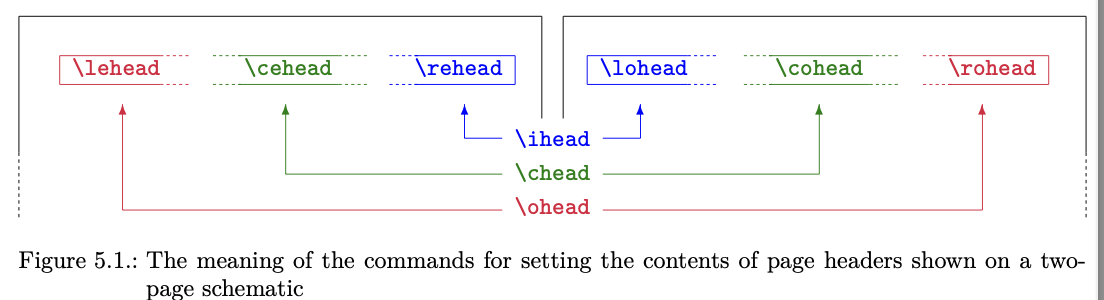
\includegraphics[width=1\linewidth]{imagem04.png}
\end{figure}

Mas o que acontece? Na primeira página, há apenas um número de página no rodapé, enquanto o cabeçalho permanece vazio!

A explicação é simples: a classe scrartcl, como a classe de artigo padrão, muda para o estilo de página simples para a página que contém o título. Após o comando \cmd{pa\-ge\-sty\-le{scr\-head\-ings}} no preâmbulo do nosso exemplo, isso realmente se refere ao estilo de página plain.scrheadings. O padrão para este estilo de página ao usar uma classe \KOMAScript\ é um cabeçalho de página vazio e um número de página no rodapé. No exemplo, os argumentos opcionais de \cmd{lohead} e \cmd{rohead} são omitidos, então o estilo de página plain.scrheadings permanece inalterado e o resultado para a primeira página está realmente correto.

O uso explícito de \cmd{pa\-ge\-sty\-le{scr\-head\-ings}} nem é necessário. O pacote já executa este comando ao carregar, então ele define automaticamente o estilo de página para scrheadings. Isso também muda não apenas os títulos de estilo de página automaticamente para scrheadings, mas também plain para plain.scrheadings.

Agora adicione texto suficiente ao exemplo após \cmd{maketitle} para que uma segunda página seja impressa. Você pode simplesmente adicionar \cmd{use\-pa\-cka\-ge\{lip\-sum\}} ao preâmbulo do documento e \cmd{lipsum} abaixo de \cmd{maketitle}. Você verá que o cabeçalho da segunda página agora contém o autor e o título do documento como queríamos.

Para comparação, você também deve adicionar o argumento opcional para 
\cmd{lohead} e \cmd{rohead}. Altere o exemplo da seguinte forma:

\begin{verbatim}
\documentclass{scrartcl}
\usepackage{scrlayer-scrpage}
\lohead[John Doe]
{John Doe}
\rohead[Page style with \KOMAScript]
{Page style with \KOMAScript}
\begin{document}
\title{Page styles with \KOMAScript}
\author{John Doe}
\maketitle
\end{document}
\end{verbatim}

Agora você tem um cabeçalho na primeira página logo acima do próprio título. Isso porque você reconfigurou o estilo de página plain.scrheadings com os dois argumentos opcionais. Como você provavelmente sabe, seria melhor deixar esse estilo de página inalterado, pois um cabeçalho acima do título do documento é bem chato.

A propósito, como uma alternativa para configurar plain.scrheadings você poderia, se você estivesse usando uma classe \KOMAScript\ ter alterado o estilo de página para páginas que contêm cabeçalhos de título. Veja \cmd{ti\-tle\-pa\-ge\-sty\-le} na seção 3.12, página 83.
Observe que você nunca deve colocar um cabeçalho de seção ou número de seção diretamente no cabeçalho usando um desses comandos. Devido à maneira assíncrona como o TeX organiza e produz páginas, fazer isso pode facilmente resultar no número errado ou texto de cabeçalho no cabeçalho corrente. Em vez disso, você deve usar o mecanismo de marcação, idealmente em conjunto com os procedimentos explicados na próxima seção.
\begin{verbatim}
\lehead*[plain.scrheadings content ]{scrheadings content}
\cehead*[plain.scrheadings content ]{scrheadings content}
\rehead*[plain.scrheadings content ]{scrheadings content}
\lohead*[plain.scrheadings content ]{scrheadings content}
\cohead*[plain.scrheadings content ]{scrheadings content}
\rohead*[plain.scrheadings content ]{scrheadings content}
\end{verbatim}

As versões com estrela dos comandos descritos anteriormente diferem das versões comuns apenas se você omitir o argumento opcional plain.scrheadings content. Neste caso, a versão sem a estrela não altera o conteúdo de plain.scrheadings. A versão com estrela, por outro lado, usa o argumento obrigatório scrheading content para plain.scrheadings também. Então, se ambos os argumentos devem ser os mesmos, você pode simplesmente usar a versão com estrela com apenas o argumento obrigatório.

\textbf{Exemplo}: Você pode encurtar o exemplo anterior usando as versões com estrela de \cmd{lohead} e \cmd{rohead}:
\begin{verbatim}
        \documentclass{scrartcl}
        \usepackage{scrlayer-scrpage}
        \lohead*{John Doe}
        \rohead*{Estilo de página com \KOMAScript}
        \begin{document}
        \title{Page styles with \KOMAScript}
        \author{John Doe}
        \maketitle
        \end{document} 
\end{verbatim}

\begin{figure}
    \centering
    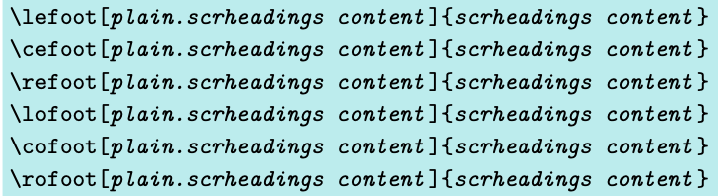
\includegraphics[width=0.8\linewidth]{imagem26.png}
\end{figure}

Você pode definir o conteúdo do rodapé para scrheadings e plain.scrheadings com estes comandos. O argumento opcional define o conteúdo de um elemento de plain.scrheadings, enquanto o argumento obrigatório define o conteúdo do elemento correspondente de scrheadings.

O conteúdo de páginas pares --- ou à esquerda --- é definido com \cmd{lefoot}, \cmd{cefoot} e \cmd{refoot}. O “e” que aparece como a segunda letra dos nomes dos comandos significa “par”.

O conteúdo de páginas ímpares --- ou à direita --- é definido com \cmd{lofoot}, \cmd{cofoot} e \cmd{rofoot}. O “o” que aparece como a segunda letra dos nomes dos comandos significa “ímpar”.

Observe que na impressão de um lado, existem apenas páginas à direita, e o \LaTeX\ as designa como páginas ímpares, independentemente do número da página.

Cada rodapé consiste em um elemento alinhado à esquerda que pode ser definido com \cmd{lefoot} ou \cmd{lofoot}. O “l” que aparece como a primeira letra dos nomes dos comandos significa “alinhado à esquerda”.

Da mesma forma, cada rodapé tem um elemento centralizado que pode ser definido com \cmd{cefoot} ou \cmd{cofoot}. O “c” na primeira letra dos nomes dos comandos significa “centralizado”.

Da mesma forma, cada rodapé tem um elemento alinhado à direita que pode ser definido com \cmd{refoot} ou \cmd{rofoot}. O “r” na primeira letra dos nomes dos comandos significa “alinhado à direita”.

No entanto, esses elementos não têm atributos de fonte individuais que podem ser alterados com os comandos \cmd{set\-ko\-ma\-font} e \cmd{add\-to\-ko\-ma\-font} (consulte a seção 3.6, página 58). Em vez disso, eles usam um elemento chamado \texttt{pa\-ge\-foot}. Antes que esse elemento seja aplicado, o elemento de fonte \texttt{pa\-ge\-head\-foot} também é aplicado. Consulte a tabela 5.1 para os padrões das fontes desses elementos.

O significado de cada comando para rodapés na impressão frente e verso é ilustrado na figura 5.2.

\textbf{Exemplo}: Vamos retornar ao exemplo do artigo curto. Digamos que você queira especificar o editor no lado esquerdo do rodapé. Você mudaria o exemplo acima para:

 \begin{verbatim}
\documentclass{scrartcl}
\usepackage{scrlayer-scrpage}
\lohead{John Doe}
\rohead{Estilo de página com \KOMAScript}
\lofoot{Smart Alec Publishing}
\usepackage{lipsum}
\begin{document}
\title{Page styles with \KOMAScript}
\author{John Doe}
\maketitle
\lipsum
\end{document}   
\end{verbatim}  

Mais uma vez, o editor não é impresso na primeira página com o título. O motivo é o mesmo do exemplo com \cmd{lohead} acima. E a solução para obter o editor na primeira página é semelhante:
\begin{verbatim}
    \lofoot[Smart Alec Publishing]{Smart Alec Publishing}
\end{verbatim}

Agora você decide que o cabeçalho e o rodapé devem usar uma fonte vertical, mas menor no lugar da fonte inclinada padrão:

\verb|\setkomafont{pageheadfoot}{\small}|

Além disso, o cabeçalho, mas não o rodapé, deve estar em negrito:

\verb|\setkomafont{pagehead}{\bfseries}|

É importante que este comando não ocorra até que scrpage-scrlayer tenha sido carregado porque a classe \KOMAScript\ define \texttt{pagehead} como um alias para \texttt{pageheadfoot}. Somente ao carregar scrpage-scrlayer o \texttt{pagehead} se tornará um elemento independente do \texttt{pageheadfoot}.

Agora adicione mais um \cmd{lipsum} e a opção \textbf{twoside} ao carregar scrartcl. Primeiro de tudo, você verá o número da página se mover do centro para a margem externa do rodapé da página, devido aos padrões alterados de scrheadings e plain.scrheadings para impressão frente e verso com uma classe \KOMAScript.

Simultaneamente, o autor, o título do documento e o editor desaparecerão da página 2. Eles só aparecem na página 3. Isso porque usamos apenas comandos para páginas ímpares. Você pode reconhecer isso pelo “o” na segunda posição dos nomes dos comandos.

\begin{figure}[h]
    \centering
    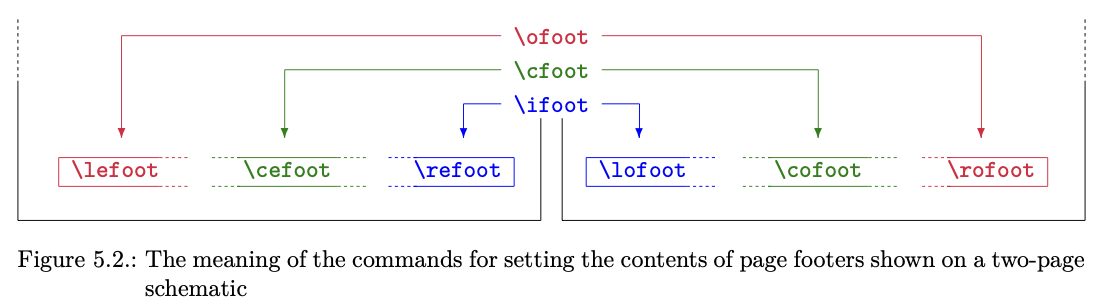
\includegraphics[width=1\linewidth]{imagem06.png}
\end{figure}

Agora, poderíamos simplesmente copiar esses comandos e substituir o “o” por um “e” para definir o conteúdo das páginas pares. Mas com a impressão frente e verso, faz mais sentido usar elementos invertidos em espelho, ou seja, o elemento esquerdo de uma página par deve se tornar o elemento direito da página ímpar e vice-versa. Para conseguir isso, também substituímos a primeira letra “l” por “r”:
\begin{verbatim}
\documentclass[twoside]{scrartcl}
\usepackage{scrlayer-scrpage}
\lohead{John Doe}
\rohead{Estilo de página com \KOMAScript}
\lofoot[Smart Alec Publishing]
{Smart Alec Publishing}
\rehead{John Doe}
\lohead{Estilo de página com \KOMAScript}
\refoot[Smart Alec Publishing]
{Smart Alec Publishing}
\usepackage{lipsum}
\begin{document}
\title{Estilos de página com \KOMAScript}
\author{John Doe}
\maketitle
\lipsum\lipsum
\end{document}
\end{verbatim}

Como é um pouco complicado definir páginas esquerda e direita separadamente em casos como o exemplo anterior, uma solução mais simples para esse caso comum é apresentada abaixo.

Permita-me mais uma vez uma observação importante: você nunca deve colocar um título de seção ou número de seção diretamente no rodapé usando um desses comandos. Devido à maneira assíncrona que o \TeX\ organiza e produz páginas, fazer isso pode facilmente resultar no número ou texto de título errado no cabeçalho corrente. Em vez disso, você deve usar o mecanismo de marcação, idealmente em conjunção com os procedimentos explicados na próxima seção.
\begin{verbatim}
\lefoot*[plain.scrheadings content ]{scrheadings content}
\cefoot*[plain.scrheadings content ]{scrheadings content}
\refoot*[plain.scrheadings content ]{scrheadings content}
\lofoot*[plain.scrheadings content ]{scrheadings content}
\cofoot*[plain.scrheadings content ]{scrheadings content}
\rofoot*[plain.scrheadings content ]{scrheadings content}  
\end{verbatim}

As versões com estrela dos comandos descritos anteriormente diferem apenas se você omitir o argumento opcional [plain.scrheadings content]. Nesse caso, a versão sem a estrela não altera o conteúdo de plain.scrheadings. A versão com estrela, por outro lado, usa o argumento obrigatório scrheading content para plain.scrheadings também.

Então, se ambos os argumentos forem iguais, você pode simplesmente usar a versão com asterisco apenas com o argumento obrigatório.

\textbf{Exemplo}: Você pode encurtar o exemplo anterior usando as versões em estrela de \cmd{lofoot} e \cmd{refoot}:
\begin{verbatim}
\documentclass[twoside]{scrartcl}
\usepackage{scrlayer-scrpage}
\lohead{John Doe}
\rohead{Estilo de página com \KOMAScript}
\lofoot*{Smart Alec Publishing}
\rehead{John Doe}
\lohead{Estilo de página com \KOMAScript}
\refoot*{Smart Alec Publishing}
\usepackage{lipsum}
\begin{document}
\title{Estilos de página com \KOMAScript}
\author{John Doe}
\maketitle
\lipsum\lipsum
\end{document} 
\end{verbatim}

\begin{verbatim}
\ohead[plain.scrheadings content ]{scrheadings content}
\chead[plain.scrheadings content ]{scrheadings content}
\ihead[plain.scrheadings content ]{scrheadings content}
\ofoot[plain.scrheadings content ]{scrheadings content}
\cfoot[plain.scrheadings content ]{scrheadings content}
\ifoot[plain.scrheadings content ]{scrheadings content} 
\end{verbatim}

Para configurar os cabeçalhos e rodapés para impressão frente e verso com os comandos descritos anteriormente, você teria que configurar os lados esquerdo e direito separadamente um do outro. Na maioria dos casos, no entanto, os lados esquerdo e direito são mais ou menos simétricos. Um item que aparece à esquerda de uma página par deve aparecer à direita de uma página ímpar e vice-versa. Elementos centralizados geralmente são centralizados em ambos os lados.

Para simplificar a definição de tais estilos de página simétricos, scrlayer-scrpage tem atalhos. O comando \cmd{ohead} corresponde a uma chamada para \cmd{lehead} e \cmd{rohead}. O comando \cmd{chead} corresponde a uma chamada para \cmd{cehead} e \cmd{cohead}. E o comando \cmd{ihead} corresponde a uma chamada para \cmd{rehead} e \cmd{lohead}. O mesmo se aplica aos comandos equivalentes para o rodapé da página. Um esboço desses relacionamentos também pode ser encontrado na figura 5.1 na página 262 e figura 5.2 na página 265.
Exemplo: Você pode simplificar o exemplo anterior usando os novos comandos:
\begin{verbatim}
\documentclass[twoside]{scrartcl}
\usepackage{scrlayer-scrpage}
\ihead{John Doe}
\ohead{Page style with \KOMAScript}
\ifoot[Smart Alec Publishing]
{Smart Alec Publishing}
\usepackage{lipsum}
\begin{document}
\title{Page styles with \KOMAScript}
\author{John Doe}
\maketitle
\lipsum\lipsum
\end{document}    
\end{verbatim}

Como a impressão unilateral trata todas as páginas como páginas ímpares, esses comandos são sinônimos dos comandos correspondentes do lado direito quando no modo unilateral. Portanto, na maioria dos casos você precisará apenas desses seis comandos em vez dos doze descritos antes.

Permita-me mais uma vez uma observação importante: você nunca deve colocar um título de seção ou número de seção diretamente no rodapé usando um desses comandos. Devido à maneira assíncrona com que o TeX organiza e produz páginas, isso pode facilmente resultar no número ou texto de título errado no cabeçalho. Em vez disso, você deve usar o mecanismo de marcação, idealmente em conjunção com os procedimentos explicados na próxima seção.
\begin{verbatim}
\ohead*[plain.scrheadings content ]{scrheadings content}
\chead*[plain.scrheadings content ]{scrheadings content}
\ihead*[plain.scrheadings content ]{scrheadings content}
\ofoot*[plain.scrheadings content ]{scrheadings content}
\cfoot*[plain.scrheadings content ]{scrheadings content}
\ifoot*[plain.scrheadings content ]{scrheadings content}
\end{verbatim}

Os comandos descritos anteriormente também têm versões com asterisco que diferem apenas se você omitir o argumento opcional [\texttt{plain.scrheadings content}]. Nesse caso, a versão sem asterisco não altera o conteúdo de \texttt{plain.scrheadings}. A versão com asterisco, por outro lado, também usa o argumento obrigatório \texttt{scrheadings content} para \texttt{plain.scrheadings}. Então se ambos os argumentos devem ser os mesmos, você pode simplesmente usar a versão com estrela com apenas o argumento obrigatório.

\textbf{Exemplo}: Você pode encurtar o exemplo anterior usando a versão com estrela de \cmd{ifoot}:
\begin{verbatim}
\documentclass[twoside]{scrartcl}
\usepackage{scrlayer-scrpage}
\ihead{John Doe}
\ohead{Estilo de página com \KOMAScript}
\ifoot*{Smart Alec Publishing}
\usepackage{lipsum}
\begin{document}
\title{Page styles with \KOMAScript}
\author{John Doe}
\maketitle
\lipsum\lipsum
\end{document} 
\end{verbatim}

\minisec{pagestyleset=setting}
Os exemplos acima se referem várias vezes às configurações padrão dos estilos de página \texttt{scrheadings} e \texttt{plain.scrheadings}. Na verdade, scrlayer-scrpage atualmente fornece dois padrões diferentes para esses estilos de página. Você pode selecioná-los manualmente com a opção \texttt{pagestyleset}.

A configuração \KOMAScript\ seleciona os padrões, que também são definidos automaticamente se a opção não for especificada e uma classe \KOMAScript\ for detectada. Na impressão frente e verso, \texttt{scrheadings} usa cabeçalhos de corrida alinhados externamente no cabeçalho e números de página alinhados externamente no rodapé. Na impressão unilateral, o cabeçalho de corrida será impresso no meio do cabeçalho e o número da página no meio do rodapé. Letras maiúsculas e minúsculas são usadas nos cabeçalhos de corrida automáticos como eles realmente aparecem nos títulos de seccionamento. Isso corresponde à opção \texttt{markcase=used}. O estilo de página \texttt{plain.scrheadings} não tem cabeçalhos correntes, mas os números de página são impressos da mesma maneira.

No entanto, se a classe \textbf{scrlttr2} for detectada, as configurações padrão serão baseadas nos estilos de página daquela classe. Veja a seção 4.13, página 230.

A configuração padrão seleciona padrões que correspondem aos estilos de página das classes padrão. Isso também é ativado automaticamente se a opção não tiver sido especificada e nenhuma classe \KOMAScript\ for detectada. Neste caso, para impressão frente e verso \texttt{scrheadings} usa cabeçalhos correntes alinhados internamente no cabeçalho, e os números de página serão impressos --- também no cabeçalho --- alinhados externamente. A impressão unilateral usa as mesmas configurações, mas como apenas páginas à direita existem neste modo, o cabeçalho corrente sempre será alinhado à esquerda e o número da página alinhado à direita. Os cabeçalhos correntes automáticos --- apesar das objeções tipográficas consideráveis --- são convertidos para letras maiúsculas, como seriam com \texttt{markcase=upper}. Na impressão de um lado, o estilo de página plain.scrheadings difere consideravelmente de \texttt{scrheadings} porque o número da página é impresso no meio do rodapé. Ao contrário do estilo de página simples nas classes padrão, \texttt{plain.scrheadings} omite o número da página na impressão frente e verso. As classes padrão imprimem o número da página no meio do rodapé, o que não corresponde ao resto dos estilos de página na impressão frente e verso. O cabeçalho é omitido em \texttt{plain.scrheadings}.

Observe que usar esta opção ativa o estilo de página \texttt{scrheadings}.


